\documentclass[10pt,a4paper]{article}
\usepackage[utf8]{inputenc}
\usepackage[T1]{fontenc}
\usepackage{amsmath}
\usepackage{amsfonts}
\usepackage{amssymb}

\usepackage{listings}
\usepackage{color}
\usepackage{tikz}
\usetikzlibrary{arrows}

\title{DD2206 - Operativsystem \\ Laboration 1 \\ Digenv - processkommunikation med pipes  v1.1 \\ Period 1, läsår 2014}
\author{Carl Svensson, F-10 \\ 910414-1412 \\ carlsven@kth.se}
\date{}

\definecolor{dkgreen}{rgb}{0,0.6,0}
\definecolor{gray}{rgb}{0.5,0.5,0.5}
\definecolor{mauve}{rgb}{0.58,0,0.82}

\lstdefinestyle{cstyle}{%
  language=C,
  aboveskip=3mm,
  belowskip=3mm,
  showstringspaces=false,
  columns=flexible,
  basicstyle={\small\ttfamily},
  numbers=none,
  numberstyle=\color{mauve},
  keywordstyle=\color{blue},
  commentstyle=\color{dkgreen},
  stringstyle=\color{mauve},
  breaklines=true,
  breakatwhitespace=true
  tabsize=3
}

\lstdefinestyle{bashstyle}{%
  language=C,
  aboveskip=3mm,
  belowskip=3mm,
  showstringspaces=false,
  columns=flexible,
  basicstyle={\small\ttfamily},
  numbers=none,
  numberstyle=\color{mauve},
  keywordstyle=\color{blue},
  commentstyle=\color{dkgreen},
  stringstyle=\color{mauve},
  breaklines=true,
  breakatwhitespace=true
  tabsize=3
}

\lstset{
  style=bashstyle
}

\begin{document}

\maketitle
\clearpage


\section{Problembeskrivning}

Uppgiften är att skriva ett program som underlättar att titta på miljövariablerna. Programmet ska motsvara att köra "printenv | grep <filter> | sort | less" i t.ex. Bash. Om inget filter anges så hoppas grep-steget över.
Programmet ska dessutom inte nödvändigtvis använda just \emph{less} utan det program som är satt som pager. Detta hittas med hjälp av PAGER-miljövariabeln. Om den inte är satt så används \emph{less} men om den inte finns så ska istället \emph{more} användas.

\subsection{Förberedelsefrågor}

\begin{enumerate}
\item Processen med pid $1$ heter \emph{init}
\item Barnprocesser ärver en kopia av föräldraprocessens alla miljövariabler vilket gör att man kan kommunicera från föräldraprocess till barnprocess med dem. Det går däremot inte att kommunicera åt andra hållet med dem.
\item Anrop till \emph{sigaction} med \emph{SIGKILL} som argument resulterar i ett felmeddelande "Invalid argument". Man-sidan specificerar tydligt att man inte kan anropa \emph{sigaction} med bland annat \emph{SIGKILL} som argument och att det i så fall genererar felkoden \emph{EINVAL}. 
\item Föräldraprocessen måste kunna veta PID till barnprocessen och får därför den från fork. Om barnprocessen behöver veta sin egen PID så kan den använda \emph{getpid} istället.
\item 
\item Anrop \emph{read} returnerar EOF om och endast om alla skriv-ändar av pipen är stängda. På motsvarande sätt returnerar \emph{write} genererar en \emph{SIGPIPE}-signal om alla läs-ändar är stängda. Om en process inte stänger den sida av pipen den inte använder kommer därför aldrig den andra sidan att kunna bli medveten om pipen har stängts från andra sidan.
\item En process som vill veta om en process med ett visst PID fortfarande lever kan anropa \emph{kill(pid, 0)} och kontrollera om det resulterar i ett fel vilket i så fall betyder att processen inte längre existerar.
\item Det finns 3 exit-koder i \emph{grep}. $0$ betyder att allt gick bra och att minst $1$ rad hittades. $1$ betyder att inget hittades och $2$ betyder att något gick fel.
\end{enumerate}

\section{Programbeskrivning}

Programmet kör en loop som går ett varv för varje delsteg i programmet, dvs. en gång för vardera barnprocess som ska startas. Varje varv görs i huvudsak fem saker:

\begin{enumerate}
\item En ny pipe skapas
\item Föräldraprocessen forkar och skapar en barnprocess
\item Barnprocessen dirigerar förra varvets pipe till sin \emph{stdin} och sin \emph{stdout} till detta varvets pipe
\item Barnprocessen exekverar det aktuella delsteget i form av någon av processerna \emph{printenv}, \emph{sort}, \emph{grep} eller \emph{less} (eller annan pager).
\item Föräldraprocessen sparar pipen för att sedan kunna användas i steg 3 i nästa varv.
\end{enumerate}

Till sist väntar föräldraprocessen på att alla barnprocesser avslutats innan den själv avslutas. Loopen har tre ytterligare detaljer som bör anmärkas. Första varvet finns det såklart ingen pipe från något tidigare varv utan då används istället \emph{stdin}. Sista varvet så dirigerar inte barnprocessen om \emph{stdout} utan behåller den som utmatning. Slutligen så hoppas \emph{grep}-steget över om programmet inte har fått några inparametrar.

Förhållandet mellan föräldraprcessen och dessbarnprocesser kan illustreras med följande diagram.

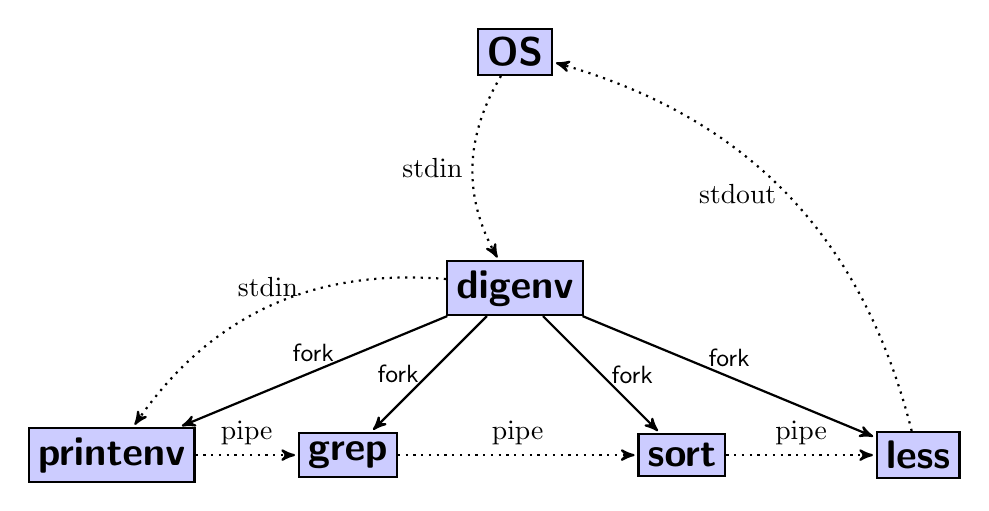
\begin{tikzpicture}[->,>=stealth',shorten >=1pt,auto,node distance=3cm,
  thick,main node/.style={rectangle,fill=blue!20,draw,font=\sffamily\Large\bfseries}]

  \node[main node] (5) {OS};
  \node[main node] (0) [below of=5] {digenv};
  \node[main node] (2) [below left of=0] {grep};
  \node[main node] (3) [below right of=0] {sort};
  \node[main node] (1) [left of=2] {printenv};
  \node[main node] (4) [right of=3] {less};

  \path[dotted]
    (5) edge [bend right] node [left] {stdin} (0)
    (0) edge [bend right] node [above] {stdin} (1)
    (1) edge node [above] {pipe} (2)
    (2) edge node [above] {pipe} (3)
    (3) edge node [above] {pipe} (4)
    (4) edge [bend right] node [left] {stdout} (5);

  \path[every node/.style={font=\sffamily\small}]
    (0) edge node [above] {fork} (1)
        edge node [left] {fork} (2)
        edge node [right] {fork} (3)
        edge node [above] {fork} (4);
    
\end{tikzpicture}

\subsection{Testkörning}

\begin{lstlisting}
$ digenv.exe HOME

> HOME=/home/calle_000
> HOMEDRIVE=C:
> HOMEPATH=\\Users\\calle\_000

$ digenv.exe COM

> COMMONPROGRAMFILES=C:\Program Files\Common Files
> COMPUTERNAME=ZETATWO
> COMSPEC=C:\WINDOWS\system32\cmd.exe
> PATHEXT=.COM;.EXE;.BAT;.CMD;.VBS;.VBE;.JS;.JSE;.WSF;.WSH;.MSC
> VS110COMNTOOLS=C:\Program Files (x86)\Microsoft Visual Studio 11.0\Common7\Tools\
> VS120COMNTOOLS=C:\Program Files (x86)\Microsoft Visual Studio 12.0\Common7\Tools\
\end{lstlisting}


\clearpage
\section{Källkod}
\lstinputlisting[style=cstyle]{../src/digenv.c}
\clearpage

\section{Arbetsgång och Utvärdering}



\end{document}